\documentclass[../main.tex]{subfiles}
\usepackage{../style}
\graphicspath{ {../img/} }
\begin{document}
    \chapter{Photoelectric Effect}
    When a beam of light strikes on surface of metals, electrons are emitted, this phenomenon is known as the photoelectric effect of light. The emitted electrons are called photoelectrons.
    \section{Experiment}
    An evacuated tube contains two electrodes connected to a source of variable voltage with the metal plate whose surface is irradiated as the anode, some of the photoelectrons that emerge from this surface have enough energy to reach the cathode despite its negative polarity and they constitute the measured current.
    \begin{figure}[ht]
        \centering
        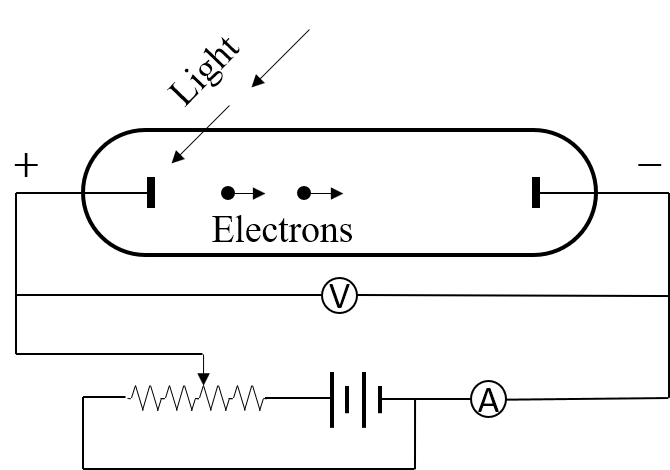
\includegraphics[scale=1]{photoelectric-experiment.png}
    \end{figure}
    The slower photoelectrons are repelled before they get to cathode. When the voltage is increased to a certain value $ v_0 $, of the order of several volts, no more photoelectrons arrive as indicated by the current dropping to zero.

    Light waves carry energy and some of the energy absorbed by the metal may somehow concentrate on individual electrons and reappear as their kinetic energy.

    \noindent\fbox{\parbox{\textwidth}{In the absence of light no electrons flow in the circuit and ammeter reads zero, because it is an open circuit.}}
    \section{Wave Theory of Light (when light behaves like a wave, not a particle)}
    If monochromatic light hits the plate behaves as a wave, wave theory of light predicts
    \begin{enumerate}
        \item If intensity of light is increased, then the number of electron emitted and their maximum kinetic energy will increase.
        \item Frequency of light does not affect kinetic energy of electrons, only the intensity does.
    \end{enumerate}
    \section{Quantum Theory of Light}
    Quantum theory of light proposed by Albert Einstein predicts that,
    \begin{itemize}
        \item A beam of light with frequency $ v $ consists of photons that each carry the same energy $ (hv) $. By increasing the intensity of beam it is possible to increase the number of photons, not the energy of each photon.
        \item According to quantum theory, a single photon collides with the electron in the metal plate. In order to emit an electron, the attractive electric forces between the electron and photon in the atom of metal plate must be overcome, that is the photon must do same amount of minimum work $ (w_0) $ to release the electron. This is known as work function.
    \end{itemize}
    If the energy carried by the photon is less than the work function electron will not be emitted.
    % \begin{tabular}[ht]{ll}
    %     If $ hv\leq w_0 $, & electrons are not emitted from metal\\ 
    %     If $ hv> w_0 $, & electrons are emitted and the remaining energy goes into the kinetic energy. 
    % \end{tabular}
    \begin{itemize}
        \item If $ hv\leq w_0 $, electrons are not emitted from metal
        \item If $ hv> w_0 $,  electrons are emitted and the remaining energy goes into the kinetic energy.
        \item $ w_0=hv_0 $ here $ v_0 $ is critical frequency below which no photoelectrons are emitted. 
    \end{itemize}
    \begin{equation*}
        \boxed{hv=k_{max}+w_0\qquad \text{or,}\qquad hv-w_0=k_{max}}
    \end{equation*}
    \begin{figure}[ht]
        \centering
        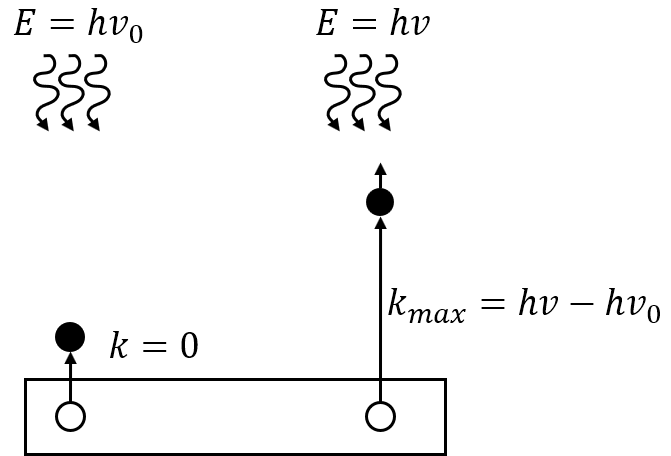
\includegraphics[scale=1]{photoenergy.png}
    \end{figure}
    \textbf{Conclusion:}
    \begin{enumerate}
        \item If the frequency of light is less than frequency required to emit electron from metal, increasing the intensity will have no effect on emitting electrons.
        \item If the frequency is large enough to emit electrons increasing the intensity increase the number of electrons emitted but $ K_{max} $ of electron will remain unchanged.
    \end{enumerate}
    \section{Compton Effect}
    The Compton effect was an experiment conducted by Arthur H. Compton in 1923 which is the further confirmation of the photon model (quantum theory of light).

    An X-ray photon strikes an electron (assumed to be initially at rest in laboratory co-ordinate system) and is scattered away from its original direction of motion while the electron receives an impulse and begins to move. If the initial photon has the frequency $ v $ associated with it, the scattered photon has lower frequency $ v' $, where,\\
    \indent Loss in photon energy = Gain in electron energy
    \begin{equation}
        hv-hv'=K_E \label{eq:comex1}
    \end{equation}
    We know, the momentum of a massless particle is related to its energy by the formula $ E=pc $.\\
    Since the energy of photon is $ hv $, its momentum is,
    \begin{equation}
        p=\frac{E}{c}=\frac{hv}{c}\label{eq:comex2}
    \end{equation}
    \begin{figure}[ht]
        \centering
        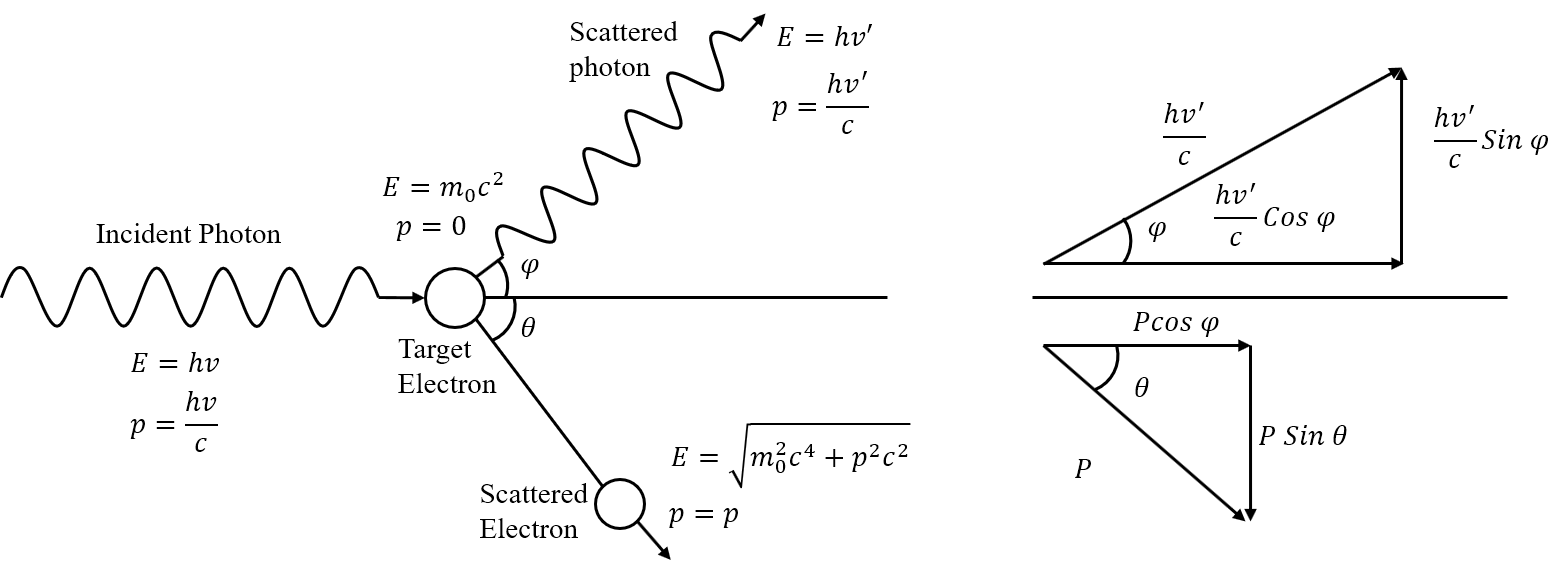
\includegraphics[scale=.75]{compton-experi.png}
    \end{figure}
    The angle $ \varphi $ is that between the directions of the initial and scattered photons and $ \theta $ is that between the directions of the initial photon and the recoil electron.\\
    Here, momentum is vector quantity. In the collision momentum must be conserved in each of two mutually perpendicular directions. The initial photon momentum is $ \frac{hv}{c} $, the scattered photon momentum is $ \frac{hv'}{c} $ and the initial and the final electron momentum are respectively $ 0 $ and $ p $.\\
    In the original photon direction:
    \begin{align}
        \text{Initial momentum} &= \text{Final momentum}\notag\\
        \frac{hv}{c}+0& =\frac{hv'}{c}\cos \varphi+p\cos\theta \label{eq:comex3}
    \end{align}
    and perpendicular to this direction:
    \begin{align}
        \text{Initial momentum} &= \text{Final momentum}\notag\\
        0& =\frac{hv'}{c}\sin \varphi-p\sin\theta \label{eq:comex4}
    \end{align}
    Multiplying equation \eqref{eq:comex3} and equation \eqref{eq:comex4} by $ c $ we get 
    \begin{align*}
        Pc \cos \theta&=hv-hv'\cos\varphi\\
        Pc \sin \theta&=hv'\sin\varphi
    \end{align*}
    Now, squaring each equation and adding then we get
    \begin{equation}
        p^2c^2=(hv)^2-2(hv)(hv')\cos\varphi+(hv')^2\label{eq:comex5}
    \end{equation}
    The total energy of a particle can be written as 
    \begin{align}
        E&=K_E+m_0c^2\label{eq:comex6}\\
        E&=\sqrt{{m_0^2}c^4+p^2c^2}\label{eq:comex7}
    \end{align}
    Now, equation \eqref{eq:comex7} can be expressed as,
    \begin{align}
        &E^2={m_0}^2c^4+p^2c^2\notag\\
        \Rightarrow\,&\left( K_E+m_0c^2 \right)^2={m_0}^2c^4+p^2c^2\notag\\
        \Rightarrow\,&p^2c^2={K_E}^2+2{m_0}c^2K_E\notag\\
        \Rightarrow\,&p^2c^2=\left( hv-hv' \right)^2+2{m_0}c^2\left( hv-hv' \right)\label{eq:comex8}
    \end{align}
    Substituting equation \eqref{eq:comex5} in equation \eqref{eq:comex8} we get,
    \begin{align}
        &(hv)^2-2(hv)(hv')\cos\varphi+(hv')^2=(hv)^2-2(hv)(hv')+(hv')^2+2m_0c^2(hv-hv')\notag\\
        \Rightarrow\,&2m_0c^2(hv-hv')=2(hv)(hv')(1-\cos\varphi)\label{eq:comex9}
    \end{align}
    Dividing equation \eqref{eq:comex9} by $ 2h^2c^2 $
    \begin{align}
        &\frac{m_0c}{h}\left( \frac{v}{c}-\frac{v'}{c} \right)=\frac{v}{c}\frac{v'}{c}\left( 1-\cos\varphi \right)\notag\\
        &\frac{m_0c}{h}\left( \frac{1}{\lambda}-\frac{1}{\lambda'} \right)=\frac{1}{\lambda}\frac{1}{\lambda'}\left( 1-\cos\varphi \right)\notag\\
        \text{or, }&\boxed{\lambda-\lambda'=\frac{h}{m_0c}(1-\cos\varphi)}\label{eq:comex10}
    \end{align}
    Equation \eqref{eq:comex10} is known as Compton effect, which shows the change in wavelength expected for a photon that is scattered through the angle $ \varphi  $ by a particle of rest mass $ m_0 $. This change is independent of wavelength $ \lambda $ of the incident photon.\\
    The quantity $ \frac{h}{m_0c}=\lambda_c $ is known as Compton wavelength
    \[\lambda'-\lambda=\lambda_c(1-\cos\varphi)\]
    For $ \varphi=180^\circ $, the wavelength change will be twice the Compton wavelength $ \lambda_c $.
    \section{Mathematical Problem}
    \begin{prob}
        UV light of wavelength $ 350 $nm and intensity $ 1.00\, W/m^2$ is directed at a potassium surface.
        \begin{enumerate}[label=(\alph*)]
            \item Find the maximum $ K_E $ of the photoelectrons.
            \item If $ 0.50 $ percent of the incident photons produce photoelectrons, how many are emitted per second if the potassium surface has an area if $ 1.00 \,cm^2 $? [work function of potassium = $ 2.2\,eV $]
        \end{enumerate}
    \end{prob}
    \begin{soln}
        \begin{enumerate}[label=(\alph*)]
            \item We know, energy of photon is
            \begin{align*}
                &E=hv\\
                \Rightarrow\,&E=h\frac{c}{\lambda}\\
                \Rightarrow\,&E=\frac{6.626\E{-34} Js}{1.602\E{-19}J/eV}\times\frac{2.998\E{8}m/s}{350\E{-9}m}\\
                \Rightarrow\,&E=3.5 \,eV
            \end{align*}
            Now,
            \[
                K_{max}=hv-\varphi=3.5\,eV-2.2\,eV=1.3eV
            \]
            \item The photon energy $ =3.5\,eV=5.68\E{-19}\,J $\\
            The number of photons that reach the surface per second is 
            \[
                h_p=\frac{E/t}{E_p}=\frac{(p/A)A}{E_p}=\frac{(1.00\,W/m^2)(1.00\E{-4}m^2)}{5.68\E{-19}}=1.76\E{14}\text{ photons/s}
            \]
            The rate at which photo electrons are emitted is therefore,
            \[n_e=(0.0050)h_p=8.8\E{11}\text{ photoelectrons/s}\]
        \end{enumerate}
    \end{soln}
    \begin{prob}
        X-rays of wavelength $ 10.0\,pm $ are scattered from a target.
        \begin{enumerate}[label=(\alph*)]
            \item Find the wavelength of x-rays scattered through $ 45^\circ $
            \item Find the maximum wavelength present in the scattered x-rays.
            \item Find the maximum kinetic energy of the recoil electrons.[$ \lambda_c=2.426\,pm $]
        \end{enumerate}
    \end{prob}
    \begin{soln}
        \begin{enumerate}[label=(\alph*)]
            \item From the equation of Compton effect we get
            \begin{align*}
                \lambda'-\lambda&=\lambda_c(1-\cos\varphi)\\
                \lambda'&=\lambda+\lambda_c(1-\cos 45^\circ)\\
                &=10.0\,pm+0.293\lambda_c\\
                &=10.7\,pm
            \end{align*}
            \item $ \lambda'-\lambda $ is a maximum when $ (1-\cos\varphi)=2\tan \varphi=180^\circ $
            \[\lambda'=\lambda+2\lambda_c=10.0\,pm+4.9\,pm=14.9\,pm\]
            \item The maximum recoil kinetic energy is equal to the different between the energies of the incident and scattered photons. So,
            \begin{align*}
                KE_{max}&=hv-hv'\\
                &=hc\left( \frac{1}{\lambda}-\frac{1}{\lambda'} \right)\\
                &=\frac{\left( 6.623\E{-34}\,Js \right)\left( 3\E{8}m/s \right) }{\E{-12}\,m/pm}\left( \frac{1}{10\,pm}-\frac{1}{14.9\,pm} \right)\\
                &=6.54\E{-15}\,pm\\
                &=40.8\,KeV
            \end{align*}
        \end{enumerate}
    \end{soln}
\end{document}